\chapter{Experiments and Applications}

In the previous two chapters the mathematical and computational challenges of image reconstruction for CT have been discussed. In chapter 3, a detailed description of a variety of different algorithms has been presented, including the ART family of algorithms, CGLS, MLEM and few TV approaches for smooth reconstruction, as well as the classic FDK reconstruction. Additionally in chapter 4 the computational aspect of CT is discussed, on where the problems computing the exact adjoint of the projection operation and mainly the computational burden of some of the operations have been mentioned. Considering the variety of available methods and the specifics of the implementation of the software developed, the TIGRE toolbox, experiments on how these algorithms compare and behave are due. Further than that, the performance of these algorithm in different experimental datasets is also an important analysis.

This chapter shows experimental analysis on both of the topics. First a variety of convergence analysis with different algorithms using synthetic data are performed, showing the differences not only between algorithms, but also between option on parameter selections. The section tries to illustrate and perhaps help build intuition on all the different parameters and options that each of these algorithms has, both within the algorithms themselves and among the different ones. Additionally some highlights on the practical challenges that the use of the algorithms entail in real applications are given.

In the second section of this chapter, a few examples of some of the algorithms are shown in different CT applications, both cone and parallel beam. Data from various different applications, from medicine to science has been tested using the TIGRE toolbox. While quantitative analysis is not possible with these datasets because the truth is not known, some insight in how the algorithms behave in each case is discussed.

\section{Algorithm Experiments}
This section experiments with a variety of algorithms and parameter within then, and shows how they behave with different synthetic data in simulation studies. 

\subsection{Convergence rates}

On chapter 3 the convergence rates of the algorithms has been mentioned, as well as computational times. Different algorithms will reach to different residuals at the same iteration, and thus understanding which ones can converge faster, thus theoretically give a better result earlier, is important. However, at the scale of the CBCT problem, faster no only means reaching a residual that is smaller in the same iterations, as the computational burden of each of the iterations also needs to be considered. And, as the backprojection operator is not exactly the adjoint of the projection operator, an effect that the classic formulation of these algorithms do not take into account can happen: divergence. All the algorithms (at least in this work) are mathematically designed to always reduce the residual each iteration, but that formulation relies on a correct adjoint operator. Thus, sometimes, when the algorithms in TIGRE have a solution very close to minimum residual solution, they may diverge. The code in the toolbox does generally check for divergence and stop, but one of the effect that can be observed is that some algorithm will always diverge in a residual that is larger than others. This means that some algorithm can, regardless of their computational times, reach to a better solution than others.

All test in this section are performed in the XCAT phantom\cite{XCAT}, in a $128^3$ voxel size and $256^2$ detector. Different number of angles are used, always uniformly distributed along the full circle. Figure \ref{fig:XCAT} shows cross sections of the phantom on its middle plane and figure \ref{fig:XCATproj} shows 3 projections of the phantom as simulated for the following tests. 

\begin{figure}[h]
\begin{center}

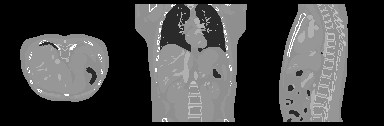
\includegraphics[width=0.9\textwidth]{Applications/XCAT.png} 
\end{center}

\caption[Cross section of the XCAT phantom]{\label{fig:XCAT} Cross section of the XCAT phantom in its middle plane in the three axis, for $128^3$ voxels.} 
\end{figure}

\begin{figure}[h]
\begin{center}

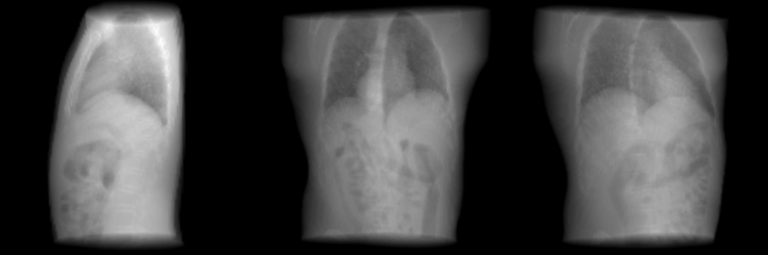
\includegraphics[width=0.9\textwidth]{Applications/XCATproj.png} 
\end{center}

\caption[Simulate projections of the XCAT phantom]{\label{fig:XCATproj} Simulate projections of the XCAT phantom in three different projection angles for a $256^2$ detector.} 
\end{figure}

\textbf{Update ordering in SART}. An analysis in the different ART-type algorithms is presented in this section first. One of the discussed parameters that has an effect in the convergence rate of the ART-type algorithms is the ordering of the used projections. Research has shown that in ART, the decrease of the residual with respect to how the rows are chosen for the updates is significantly changed[CITE], however in the algorithms feasible for big scale tomography, this effect is seen in a smaller scale. Figure \ref{fig:SARTanglesconv} shows the convergence of SART during 150 iterations using 100 projections as data. The same configuration of SART is run using ordered, randomly ordered and angular distance maximizing ordering schemes for the update order. While minor, the figure shows how random ordering does generally increases the convergence rate of the algorithm, at no computational cost. This is the default value in the software. Note that in this test there is no reduction of the relaxation parameter $\lambda$.


\begin{figure}[H]
\begin{center}

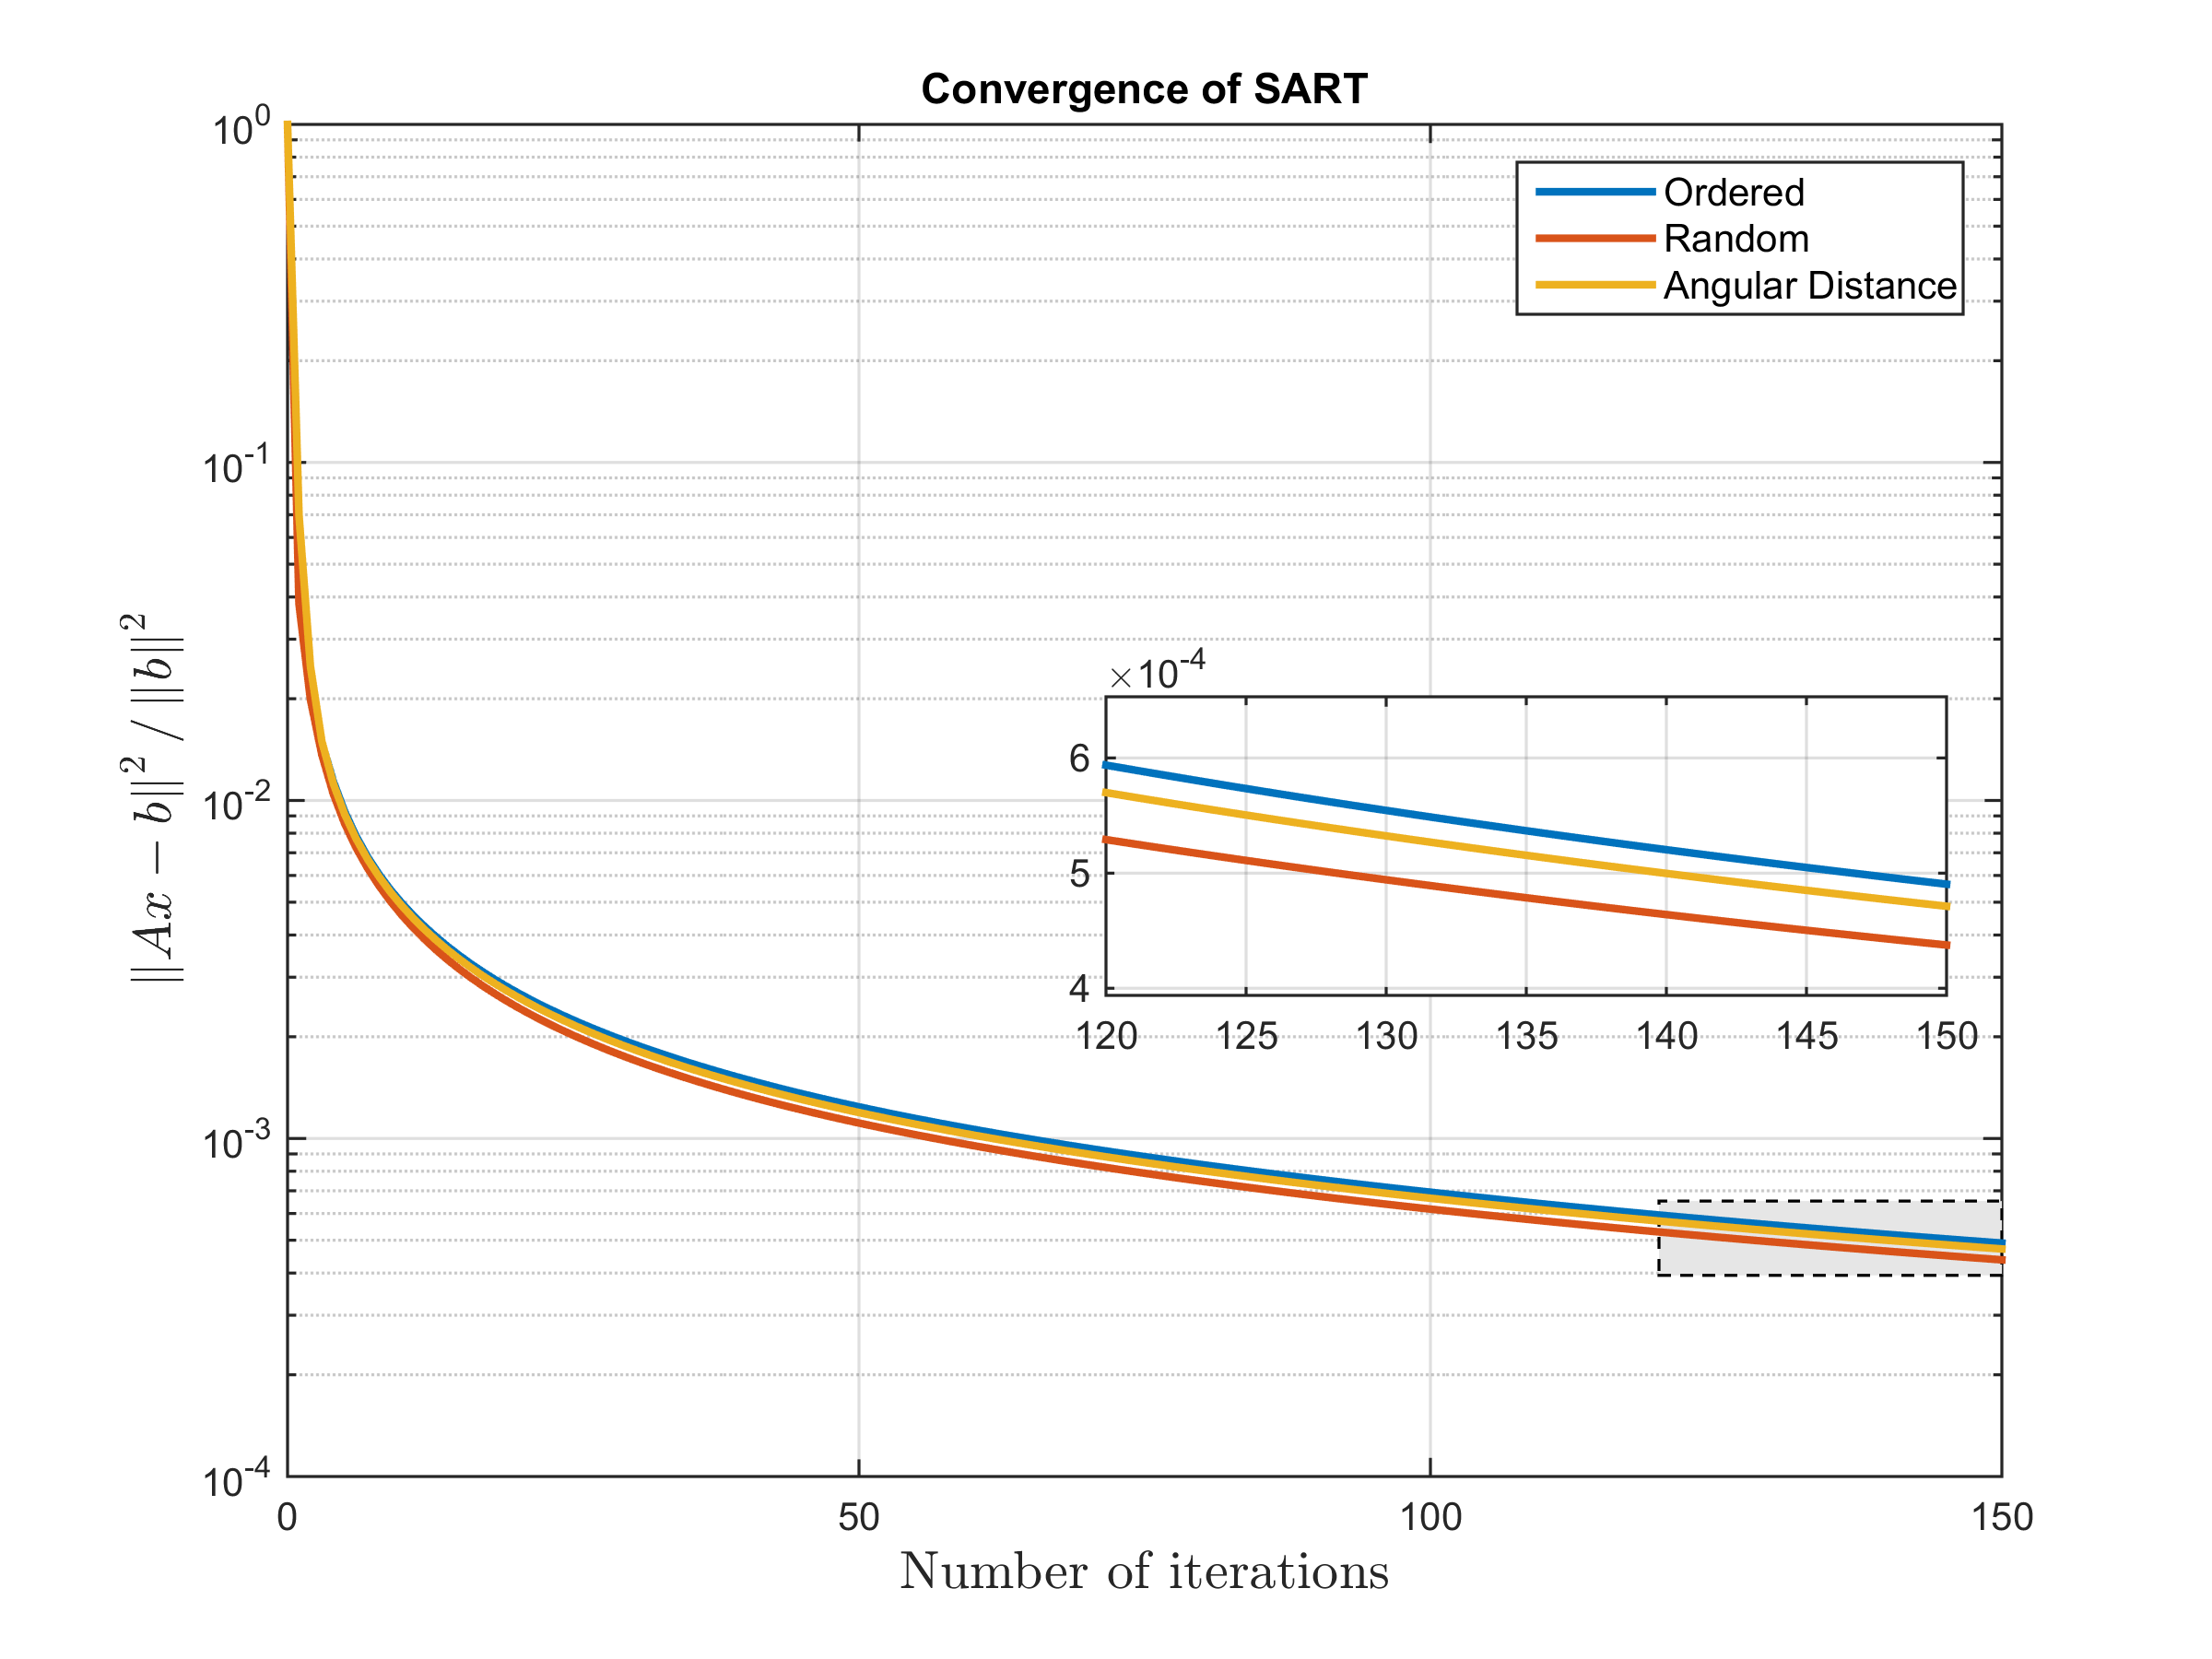
\includegraphics[width=0.8\textwidth]{Applications/SARTangles.png} 
\end{center}

\caption[Nomralized residual vs iteration of SART vs projection update order]{\label{fig:SARTanglesconv} Normalized residual versus iteration of SART compared to different angle ordering schemes, using 100 projections and no relaxation parameter reduction} 
\end{figure}

\textbf{Comparison between SART, OS-SART and SIRT}. These algorithms have very different convergence, as updating the image per-equation has the effect of converging faster. However, the computational times are greatly reduced by updating more rows at the same time. This effect can be seen in figure \ref{fig:SARTtypesconv}, on where the convergence versus iteration of these three algorithms is plotted. Note the convergence difference between SART and SIRT, where SIRT doesn't reach SART's residual even after 1000 iterations, however, each iteration of SIRT is two orders of magnitude faster than SART. OS-SART provides a middle ground alternative. Due to the specifics of the acceleration procedures for backprojection, OS-SART speeds are closer to SIRT than to SART (i.e. the speed does not change linearly with the image updates per iteration), however it is more prone to divergent behaviour in TIGRE. In the figure, OS-SART stops converging after 48 iterations. Of course, this behaviour is very data-specific, and there are multiple cases where it does not diverge. Figure XX shows the result images of these three algorithms after 150 iterations (48 for OS-SART). Note that the example being show is low data, so even in the best case, the images are slightly noisy.



\begin{figure}[H]
\begin{center}

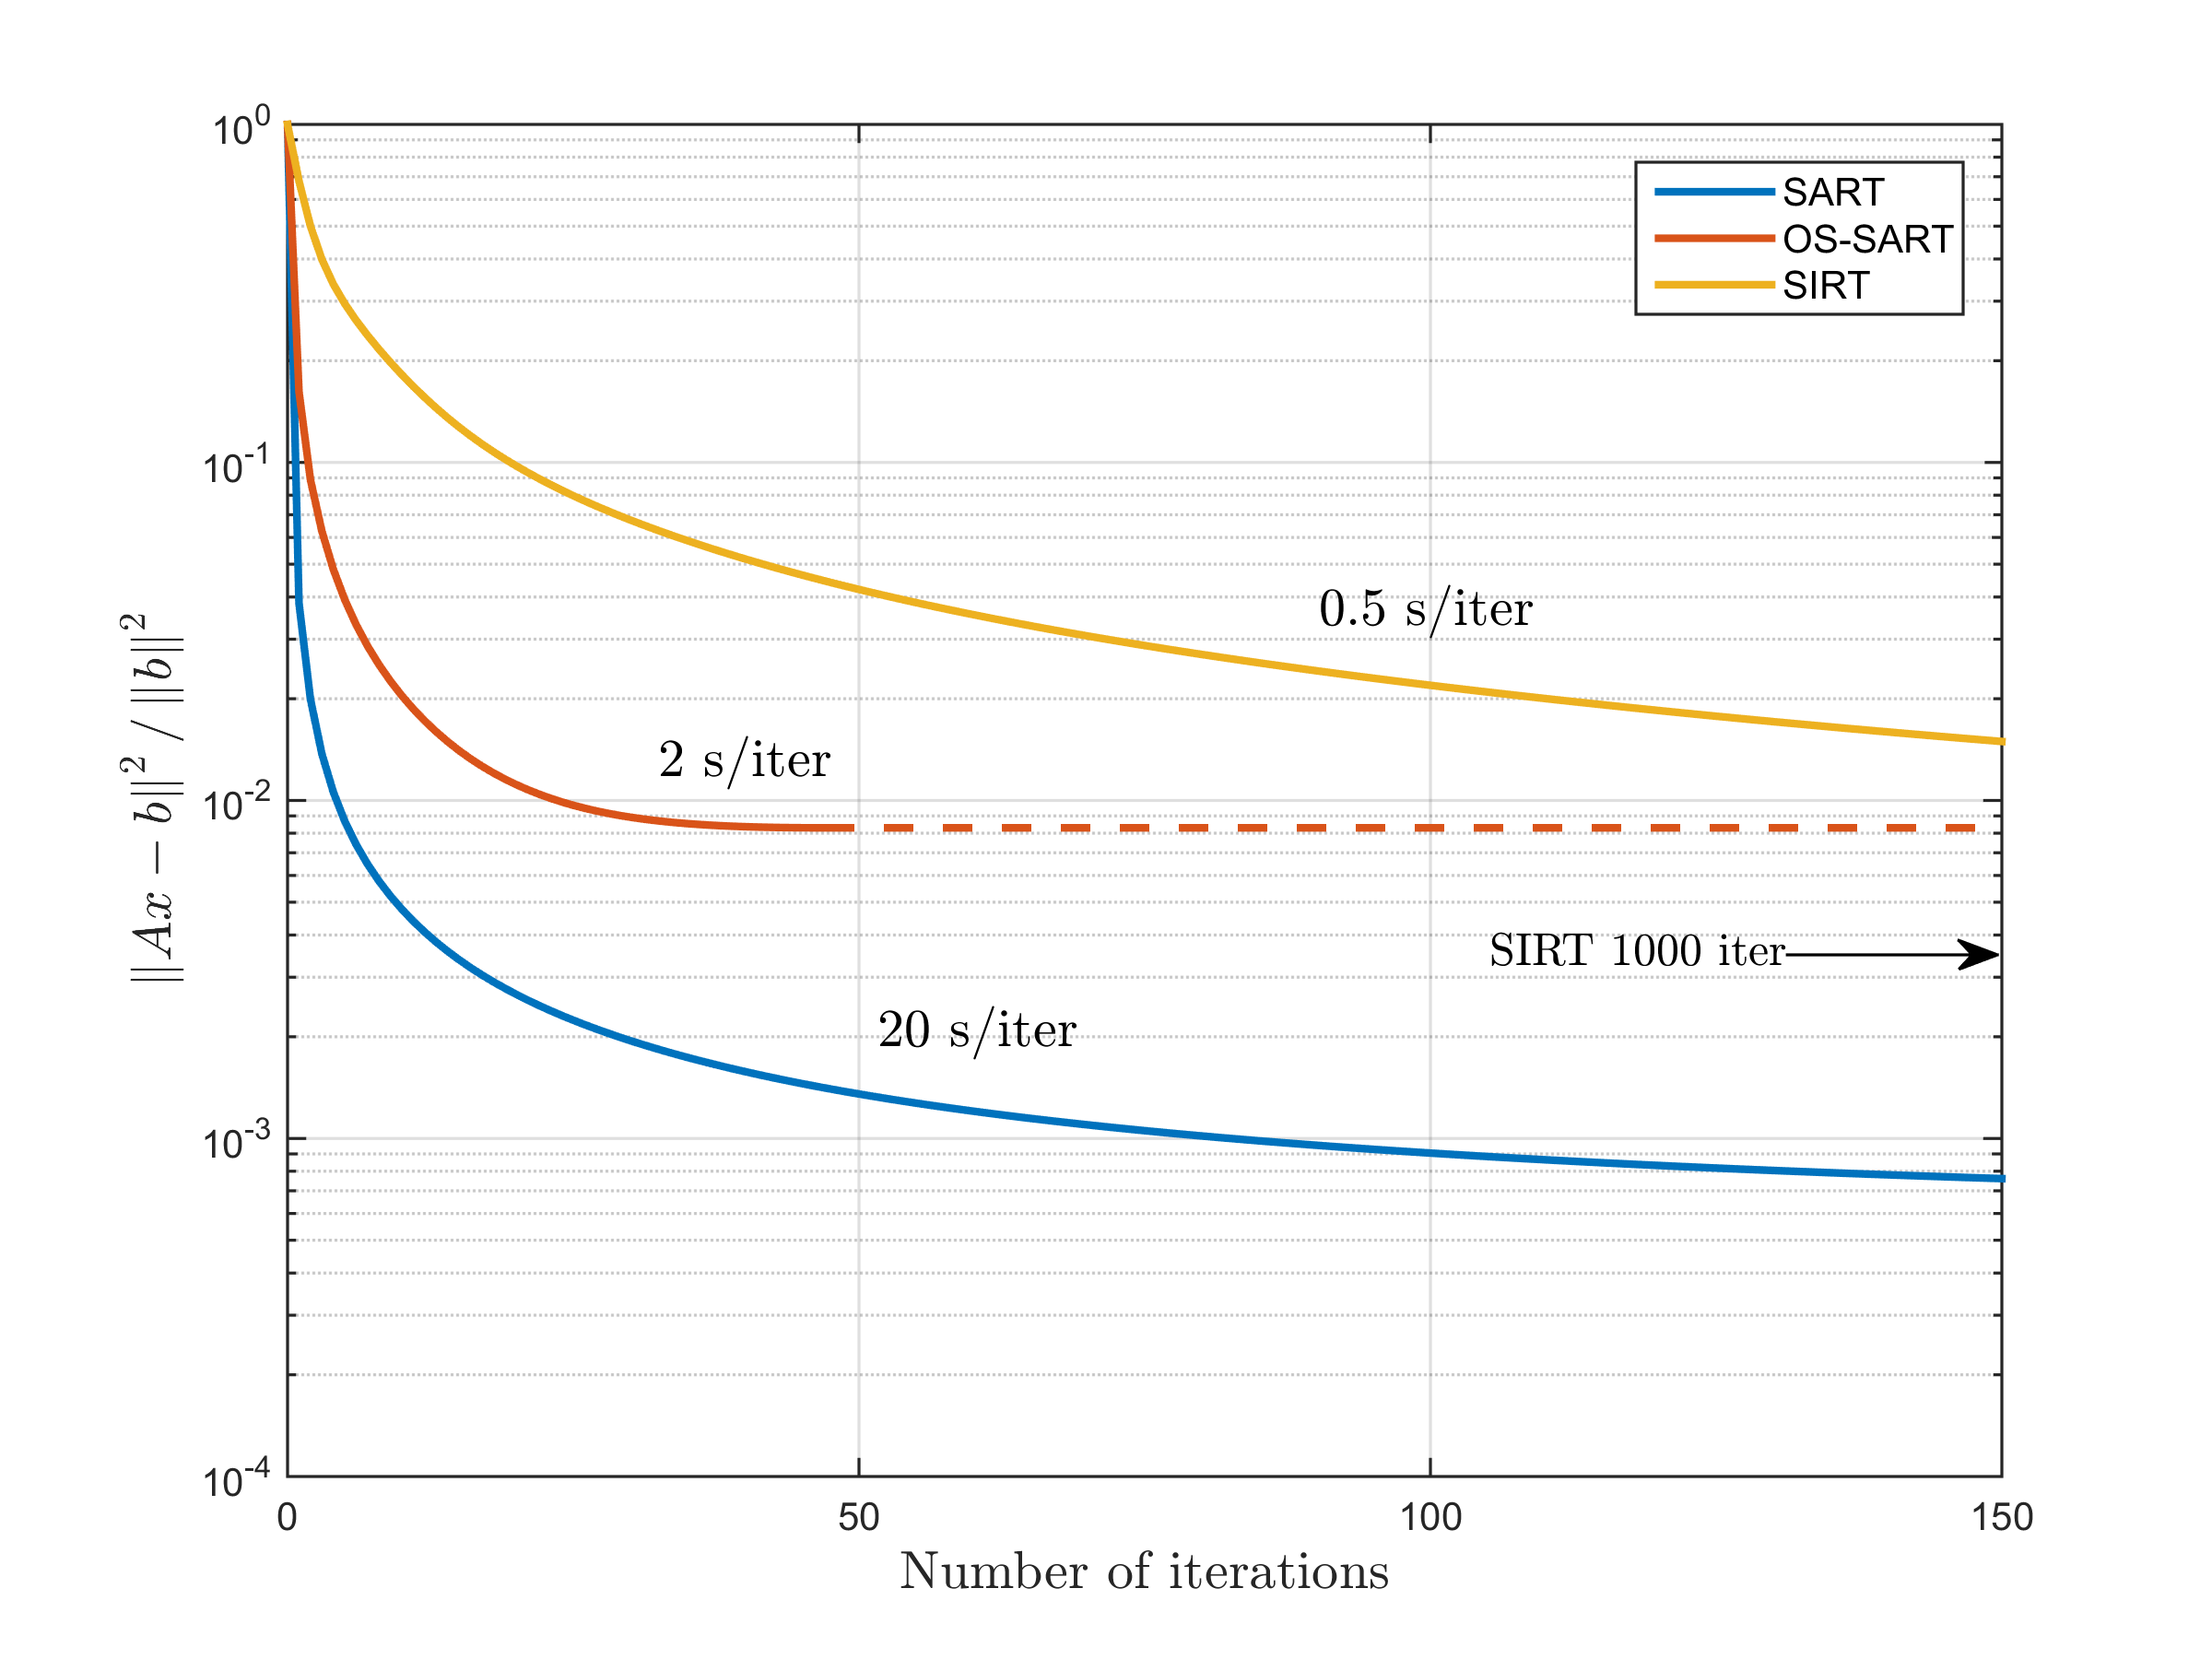
\includegraphics[width=0.8\textwidth]{Applications/SARTtypes.png} 
\end{center}

\caption[Nomralized residual vs iteration of SART/OS-SART/SIRT]{\label{fig:SARTtypesconv} Normalized residual vs iteration number for SART, OS-SART and SIRT using 100 projections and no relaxation parameter reduction.} 
\end{figure}

\textbf{Relaxation parameter.} The choice of a proper relaxation parameter does significantly change the speed on which a solution is found, and can avoid infinitely iterating through the same hyperplanes in case of an under determined or noisy solution. In TIGRE, two methods are present, as described in chapter 2: multiplying the relaxation parameter by a reduction factor after each iteration, and the Nesterov accelerated update, that does not technically update the relaxation parameter, but updates the image in each iteration using a iteration specific combination ration of the gradients of the current and previous iteration. It requires more memory, as it needs one extra image-sized variable to store the previous update, but the the algorithm finds a solution considerably faster, as it can be seen in figure \ref{fig:SARTlambda}. In the figure each of the SART, OS-SART and SIRT algorithms residual is plotted, and in each of them three versions are displayed, no relaxation parameter update, reduction with $r_{red}=0.99$ and Nesterov update. In the plot it can also be seen that reducing the relaxation parameter by a ratio, while a good approach in SART-based hybrid algorithms, such as the TV minimizing ones in TIGRE, leads with slower residual reduction and ultimately with a worse image.

In figure \ref{fig:SARTlambdaplot}, the solution found by the three algorithms using reduction of the relaxation parameter, using a Nesterov update and using static relaxation parameter of $\lambda=1$ can be seen side to side . The superior solution found by Nesterov is visually clear, and both SART and OS-SART reach a minimum in very few iterations. While SART does reach a better image (both in residual and error) without using Nesterov's update, the difference is minimal. It is important to note that using Nesterov's update, likely due to its fast convergence, leads to a faster divergent behaviour by the algorithms, thus the residual needs to be checked in each iteration leading to some computational overheat.

\begin{figure}[H]
\begin{center}

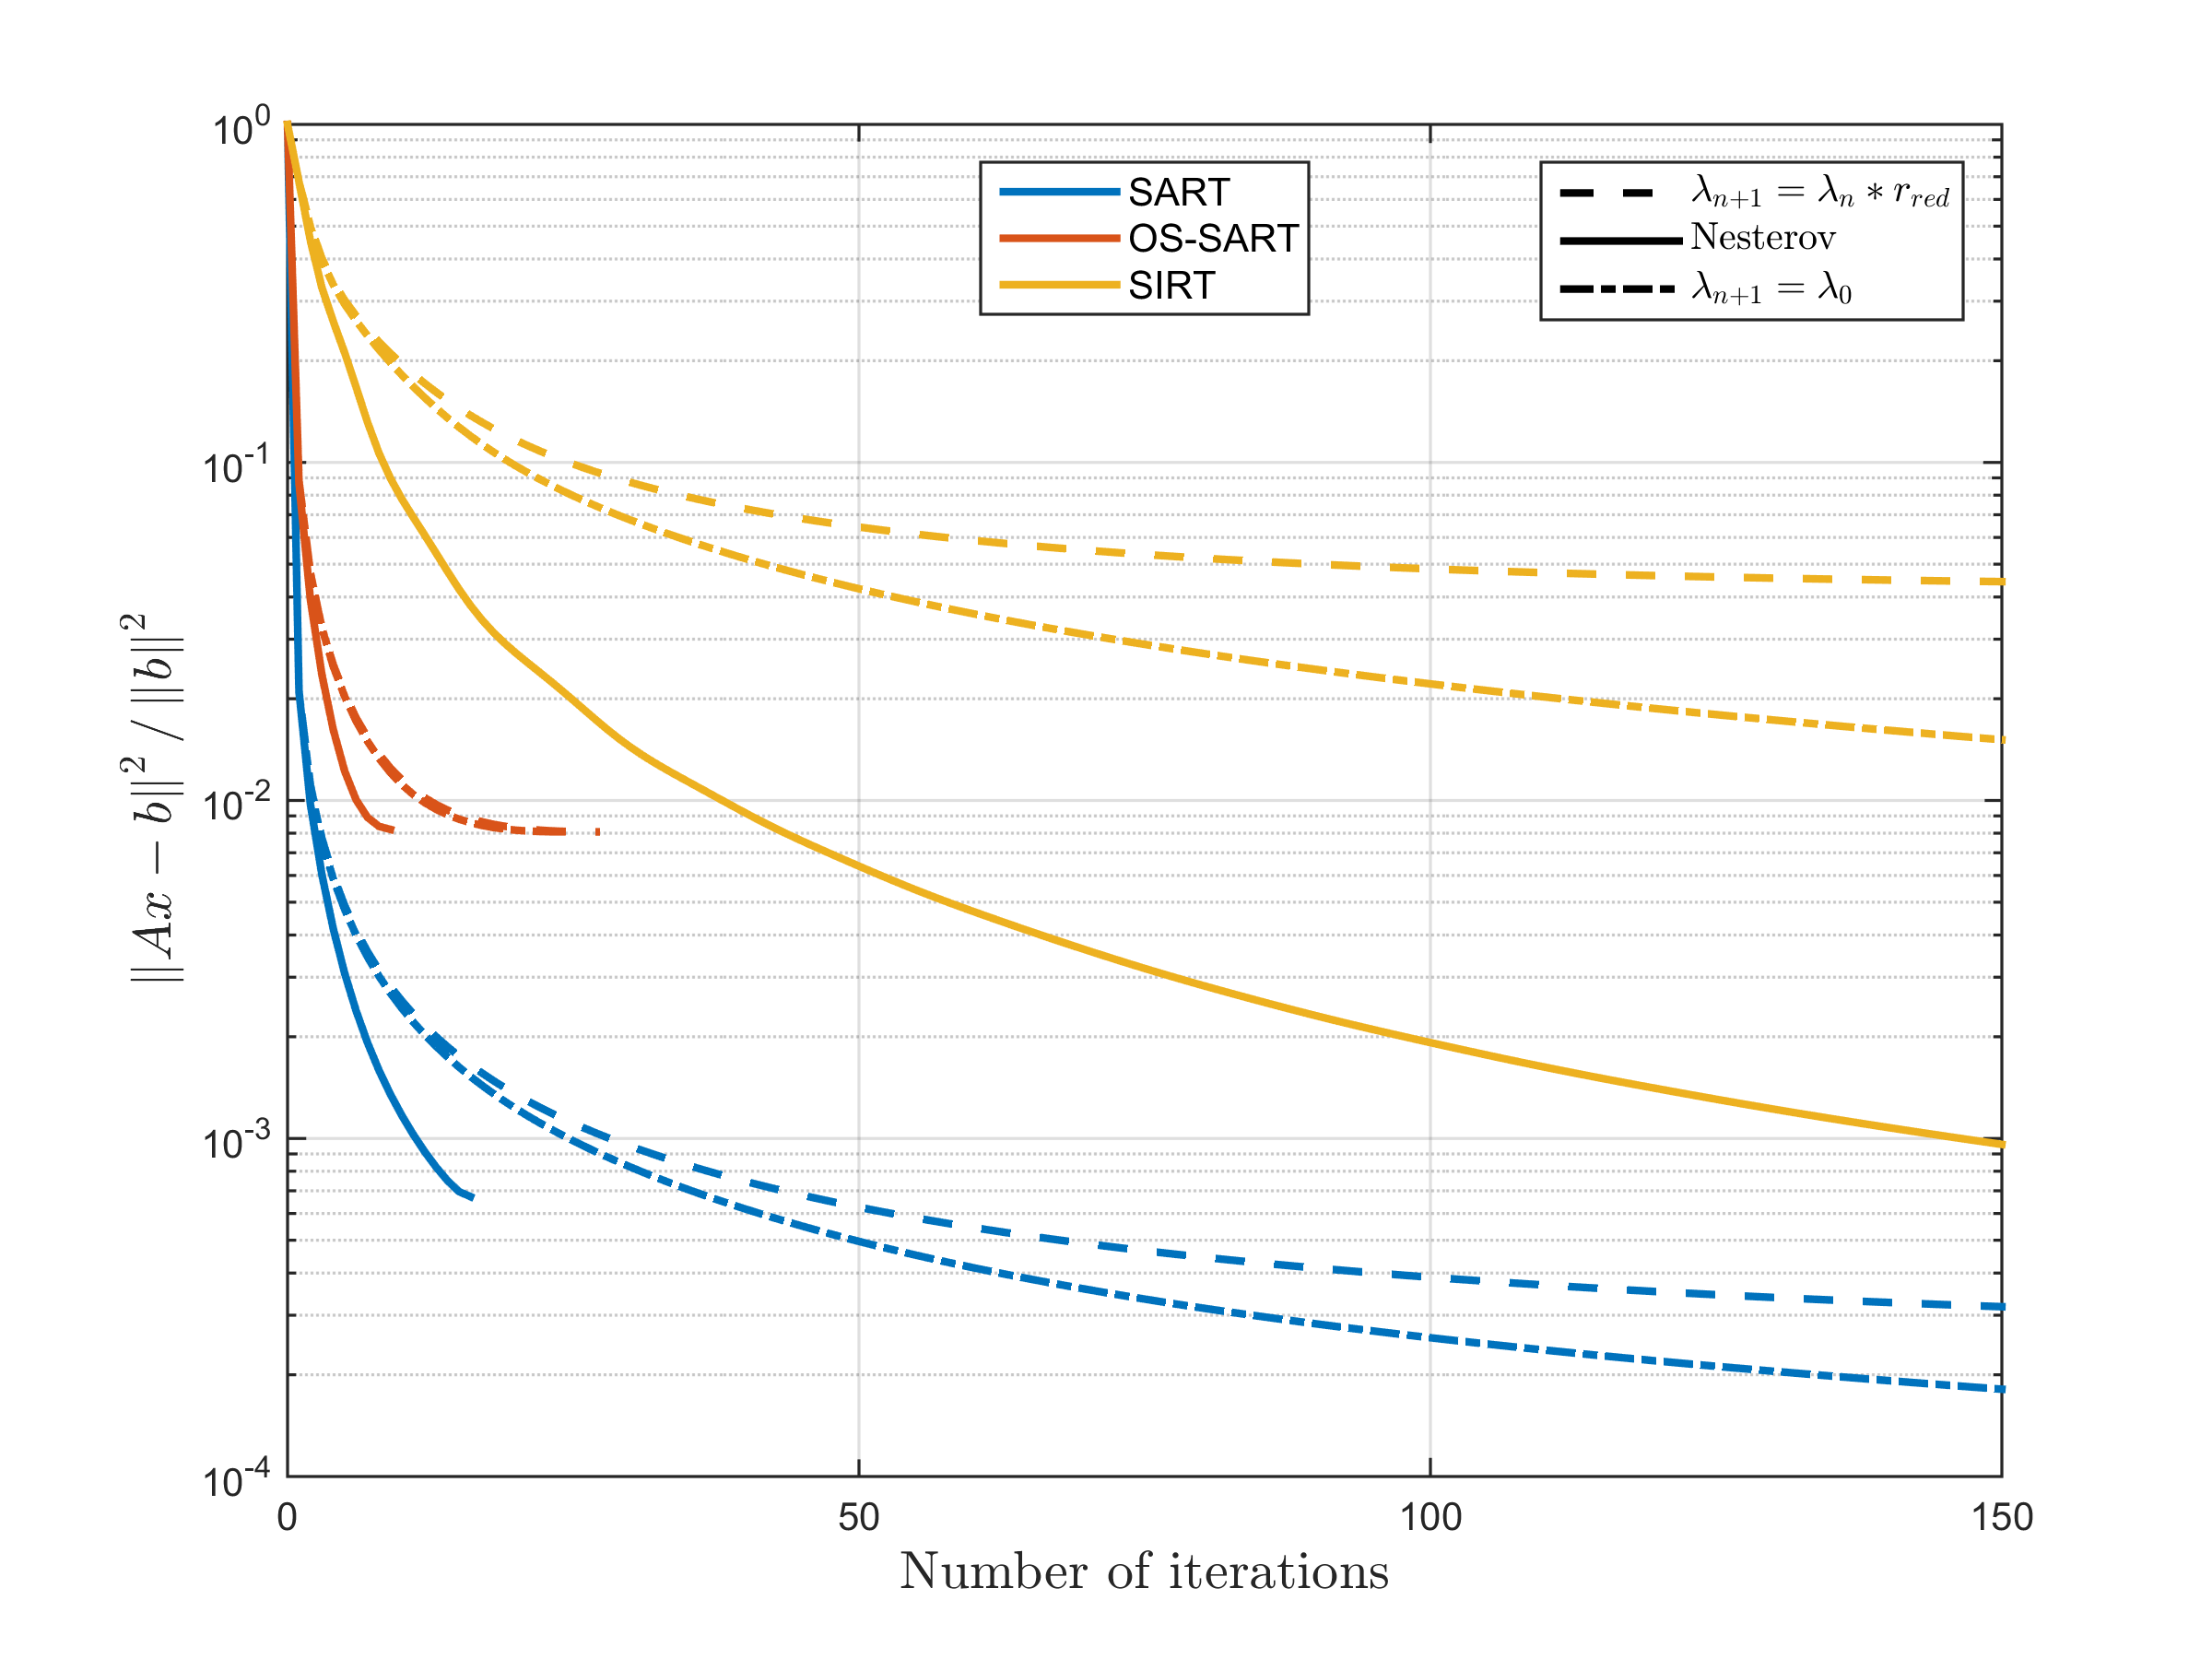
\includegraphics[width=0.8\textwidth]{Applications/SARTlambda.png} 
\end{center}

\caption[Nomralized residual vs iteration of SART/OS-SART/SIRT with different relacation parameters]{\label{fig:SARTlambda} Normalized residual vs iteration number for SART, OS-SART and SIRT using 100 projections and different relaxation parameter reduction modes. If the relaxation parameter is reduced by a constant ratio the residual reduction worsens, and if reduced using Nesterovs update, it converges very fast.} 
\end{figure}


\begin{figure}
\centering
\begin{tikzpicture}

\node (A) {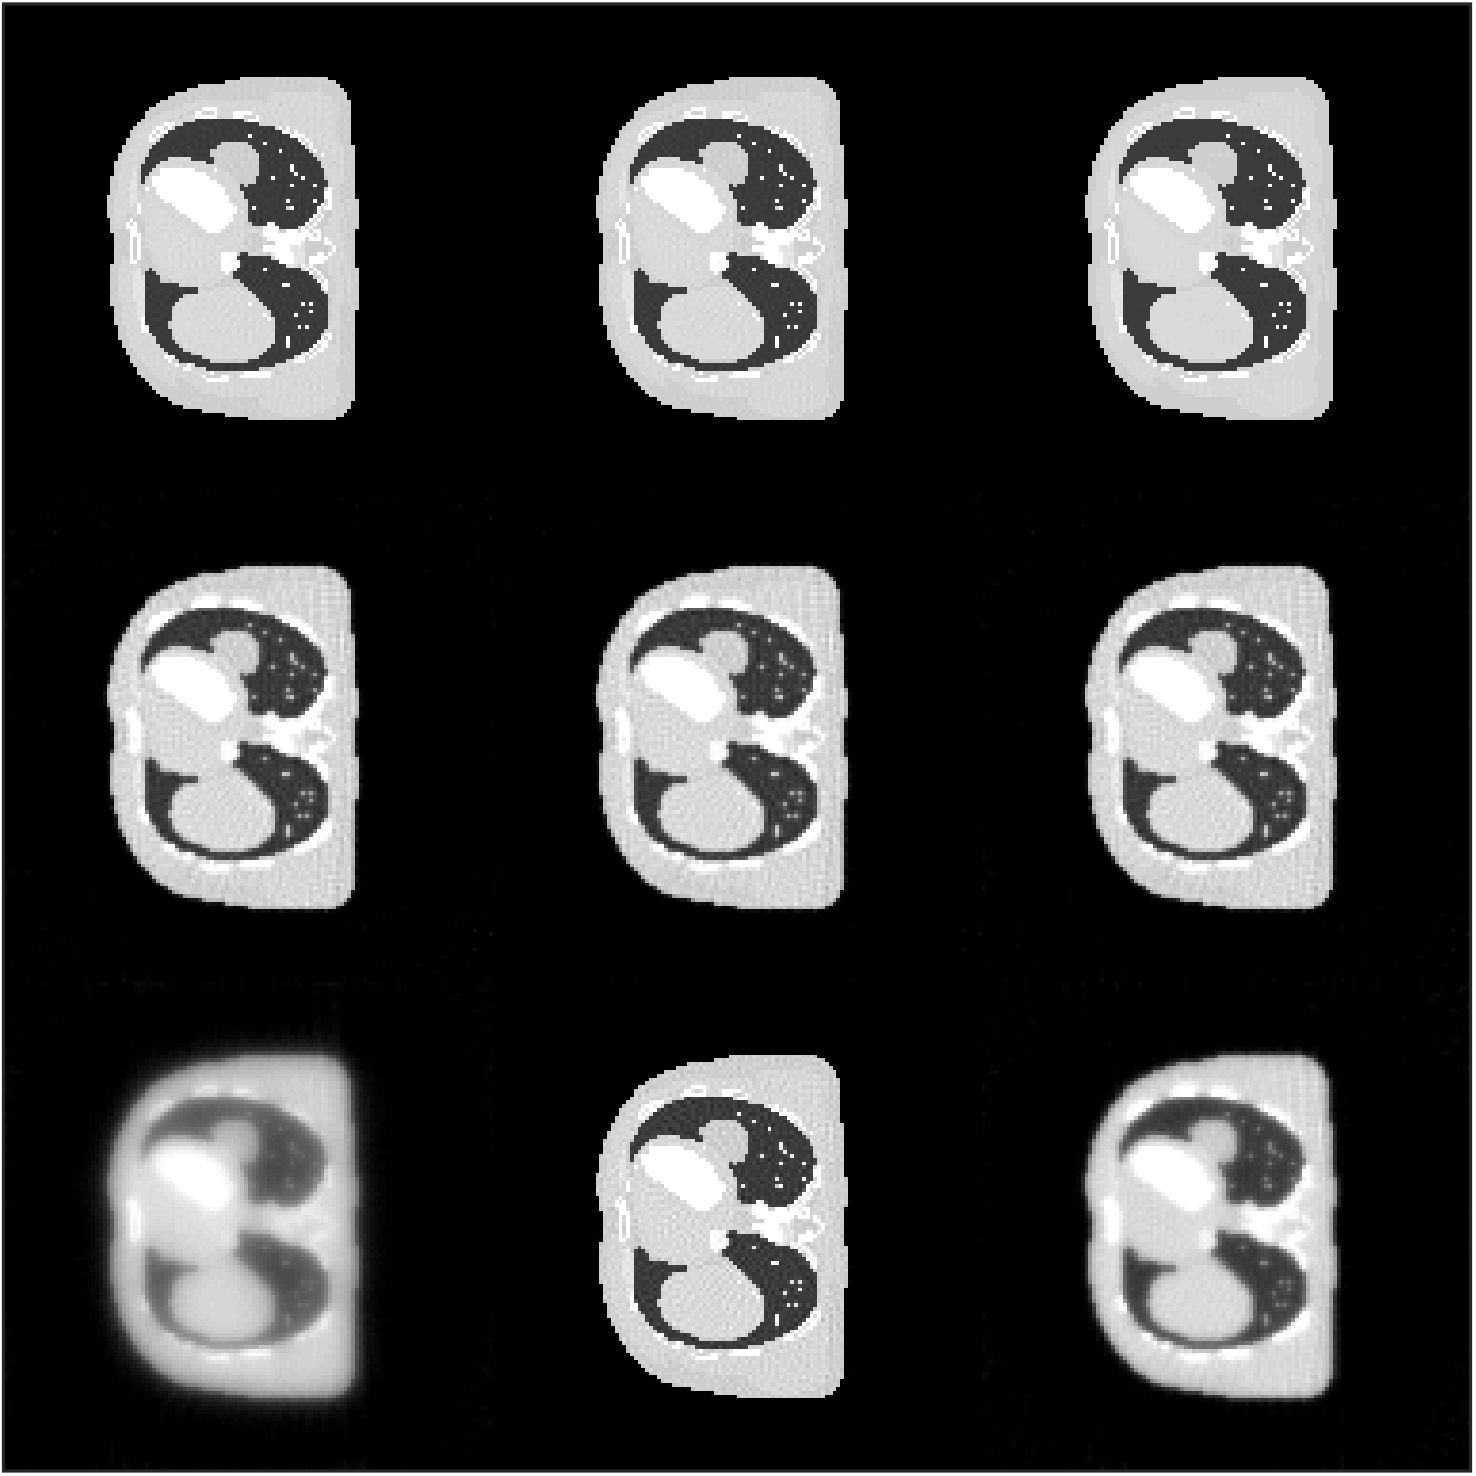
\includegraphics[width=0.94\textwidth]{Applications/SARTlambdaplot.png} };
\path (A.south west) -- (A.north west) node[pos=.18, above, rotate=90] {SIRT} node[pos=.5, above, rotate=90] {OS-SART} node[pos=.82, above, rotate=90] {SART};
\path (A.south west) -- (A.south east) node[pos=.18, below] {$\lambda_{n+1}=\lambda_{n}*r_{red}$} node[pos=.5, below] {Nesterov} node[pos=.82, below] {$\lambda_{n+1}=\lambda_0=1$};

\end{tikzpicture}
\caption[Reconstructed images with different relaxation parameter updates]{\label{fig:SARTlambdaplot}Reconstructed images with different relaxation parameter updates. OS-SART stops at iteration 24 in all but in the Nesterov case, where it stops in the iteration number 9. SART stops at iteration number 16 for Nesterov.}
\end{figure}



\subsection{Total variation minimization}
There are 4 total variation minimizing algorithms in TIGRE, with 2 different minimization functional in total. As previously described, ASD-POCS, OS-ASD-POCS and b-ASD-POCS-$\beta$ minimize the TV using a POCS minimization technique by minimizing the data constrain and TV norm independently using gradient descend. SART-TV however uses the ROF model for the TV-minimization step. The total variation algorithms are designed for applications on where the image is piecewise-smooth, as they will try to minimize the gradient on the image, by creating single valued patches in the image. In CT, the most noisy images are reconstructed when either the data is very noisy (generally due to small acquisition times and/or low energy X-rays) or when the data is limited, either from limited angle or more importantly limited amount of projections. 

An example of the behaviour of the TV algorithms with the same dataset as in figures \ref{fig:XCAT} and \ref{fig:XCATproj} is shown in figure \ref{fig:TVXCAT}. In this case, 30 uniformly sampled projections are used, perturbed with Poisson and Gaussian noise, to simulate photon scattering and electronic noise respectively. The figure shows FDK and OS-SART reconstructions, and the 4 mentioned TV algorithms. It is visually clear that the TV algorithms do provide a smoother reconstruction, and with less Normalized root mean squared error (NRMSE), as seen in table \ref{tab:NRMSE TVs}.
The reconstruction by FDk is plagued with noise, and while the main structural features can be seen, most of the detail is lost. Even the bones themselves are practically indistinguishable from noise. OS-SART does reconstruct a smoother image, something predictable as it minimizes de 2-norm, and while one can see the more details in the image, it is still low. The rest 4 TV algorithms can be seen to flatten out the attenuation levels to similar values, thus reducing most of the noise. Additionally most of the features get clearly separated from the attenuation levels of the surrounding tissues and some of the algorithms (such as ASD-POCS) are able to reconstruct even single wide pixel structures correctly. It is important to note that while the parameters used to tune this specific TV reconstruction (available in the demo number 9 in the TIGRE toolbox), they are far from optimal and very sensitive\cite{Vee}. When choosing the exact optimal parameters for the TV reconstruction algorithms, the result images tend to be significantly better than the ones shown here, but the parameter space is very data dependant and massive, thus to the author's knowledge, no parameter selection method has been proposed in the literature. 


\begin{figure}
\centering
\begin{tikzpicture}

\node (A) {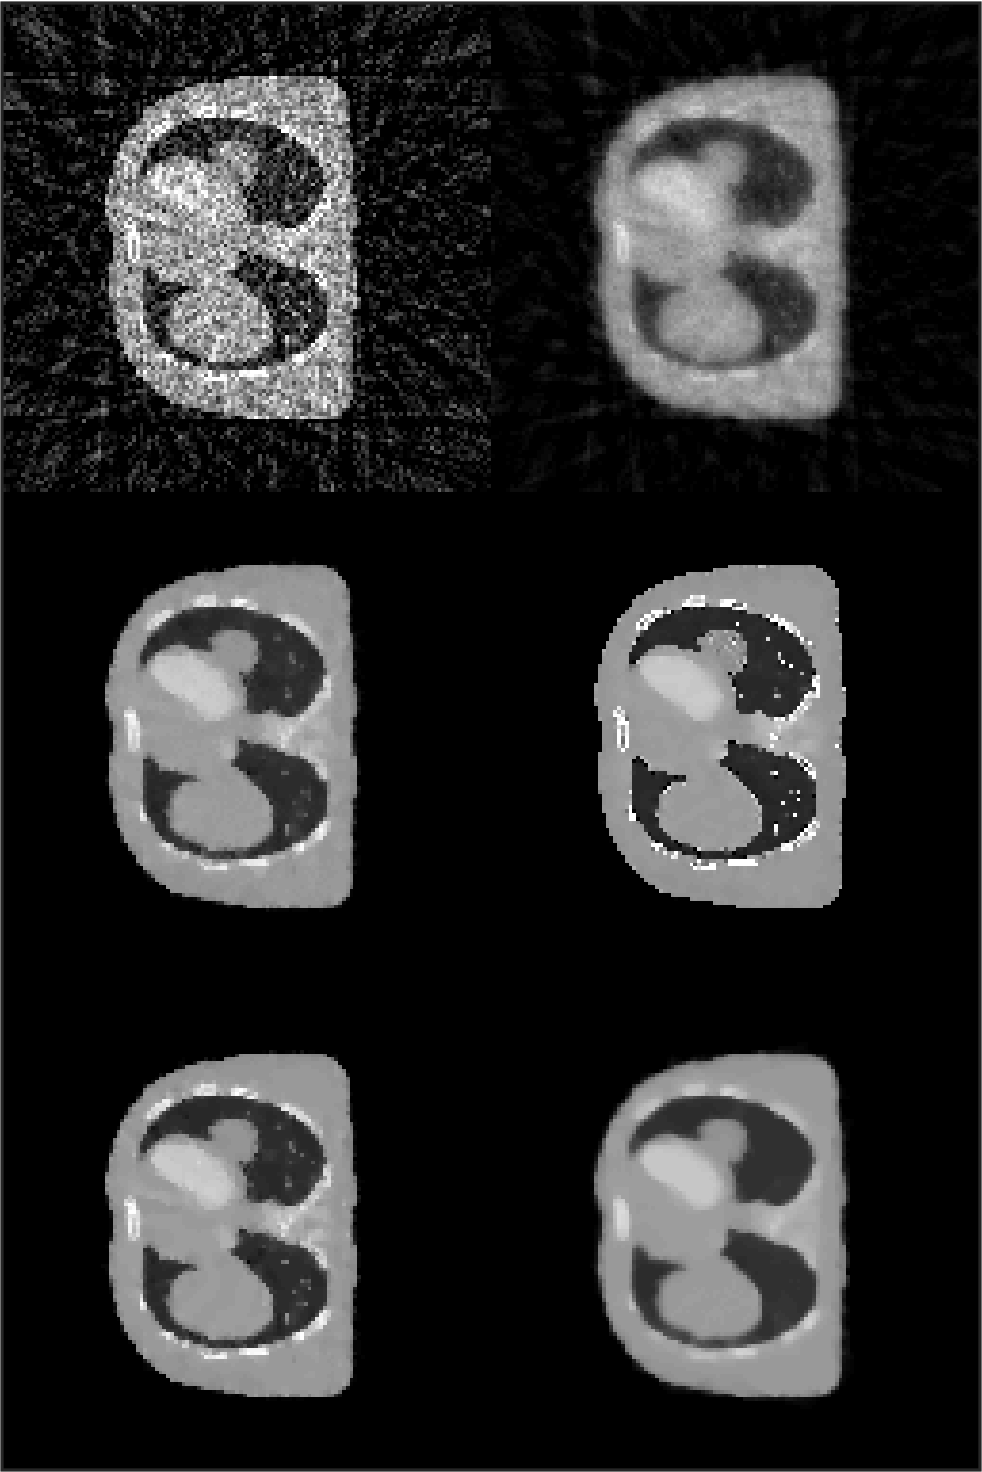
\includegraphics[width=0.4\textwidth]{Applications/TVs.png} };
\path (A.south west) -- (A.north west) node[pos=.18, above, rotate=90] {ASD-POCS} node[pos=.5, above, rotate=90] {b-ASD-POCS-$\beta$} node[pos=.82, above, rotate=90] {FDK};
\path (A.south east) -- (A.north east) node[pos=.18, below, rotate=90] {OS-ASD-POCS} node[pos=.5, below, rotate=90] {SART-TV} node[pos=.82, below, rotate=90] {OS-SART};

\node (B)at (0.5\textwidth,0) {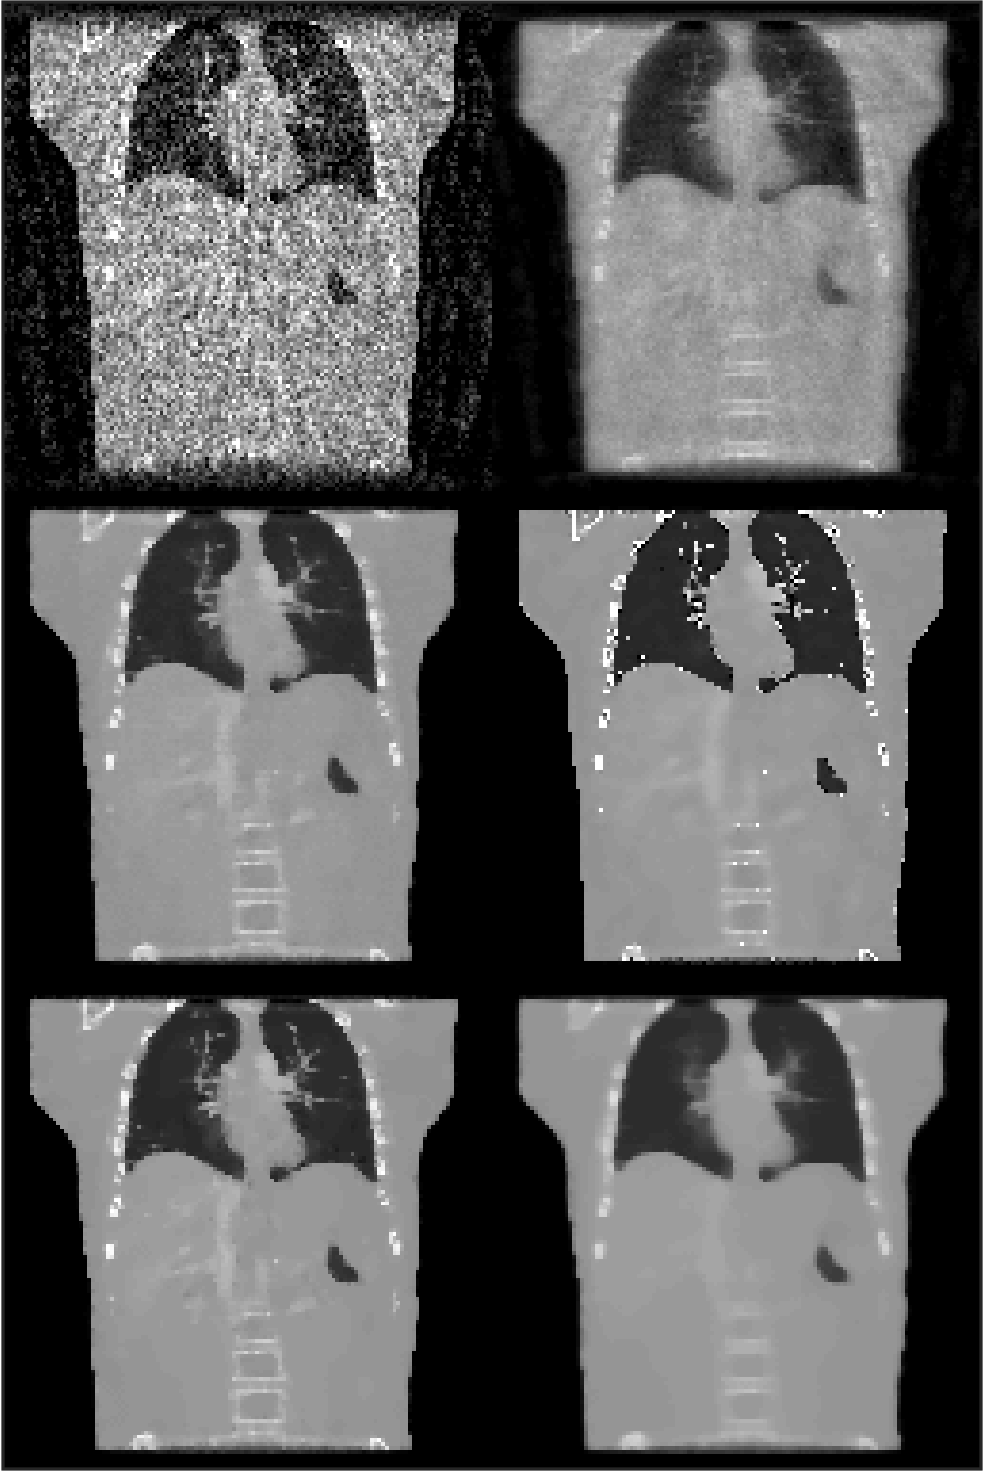
\includegraphics[width=0.4\textwidth]{Applications/TVs2.png} };
\path (B.south west) -- (B.north west) node[pos=.18, above, rotate=90] {ASD-POCS} node[pos=.5, above, rotate=90] {b-ASD-POCS-$\beta$} node[pos=.82, above, rotate=90] {FDK};
\path (B.south east) -- (B.north east) node[pos=.18, below, rotate=90] {OS-ASD-POCS} node[pos=.5, below, rotate=90] {SART-TV} node[pos=.82, below, rotate=90] {OS-SART};

\end{tikzpicture}
\caption[Reconstructed images using TV algorithms]{\label{fig:TVXCAT}Reconstructed images using FDK, OS-SART and the TV algorithms b-ASD-POCS-$\beta$, SART-TV,  ASD-POCS and OS-ASD-POCS with a limited amount and noisy data. Both figures show the same data and algorithms, but with a different cross-section of the image.}
\end{figure}


\begin{table}
\begin{center}
\caption{NRMSE for the reconstructed images in figure \ref{fig:TVXCAT}}
\label{tab:NRMSE TVs}
\scalebox{0.85}{
\begin{tabular}{| l || c | c | c | c | c | c |}
\hline
& FDK & OS-SART &b-ASD-POCS-$\beta$&SART-TV& ASD-POCS& OS-ASD-POCS\\  
\hline
\hline
NRMSE&  0.1373  &  0.0678  &  0.0338   & 0.0267 &   0.0304 &   0.0442\\   

\hline  
\end{tabular}
}
\end{center}
\end{table}






To illustrate the sensitivity to parameter selection, the algorithm SART-TV is run with 3 different values for number of TV-iterations per SART iteration for the same data set used in the previous test. The results can be seen in figure \ref{fig:SARTTVparams}, where one can clearly see how a small changes can have a devastating effect in the output image.   If a few more TV iterations are added to (b), the image gets a bit smoother and some detail is lost, as expected. However, if few iterations are removed from (b), the image can get completely destroyed. Note that these values are only applicable to this image with the exact amount of noise and projections. Different experiments may not show this behaviour or may be more intolerant to parameter change. This is arguably the biggest limitation for the common use of TV algorithms in real application. As an advantageous point, once the good parameters are found, generally the algorithm will perform similarly in similar images, thus application specific parameters may be an option.






\begin{figure}
\centering
\begin{tikzpicture}

\node (A) {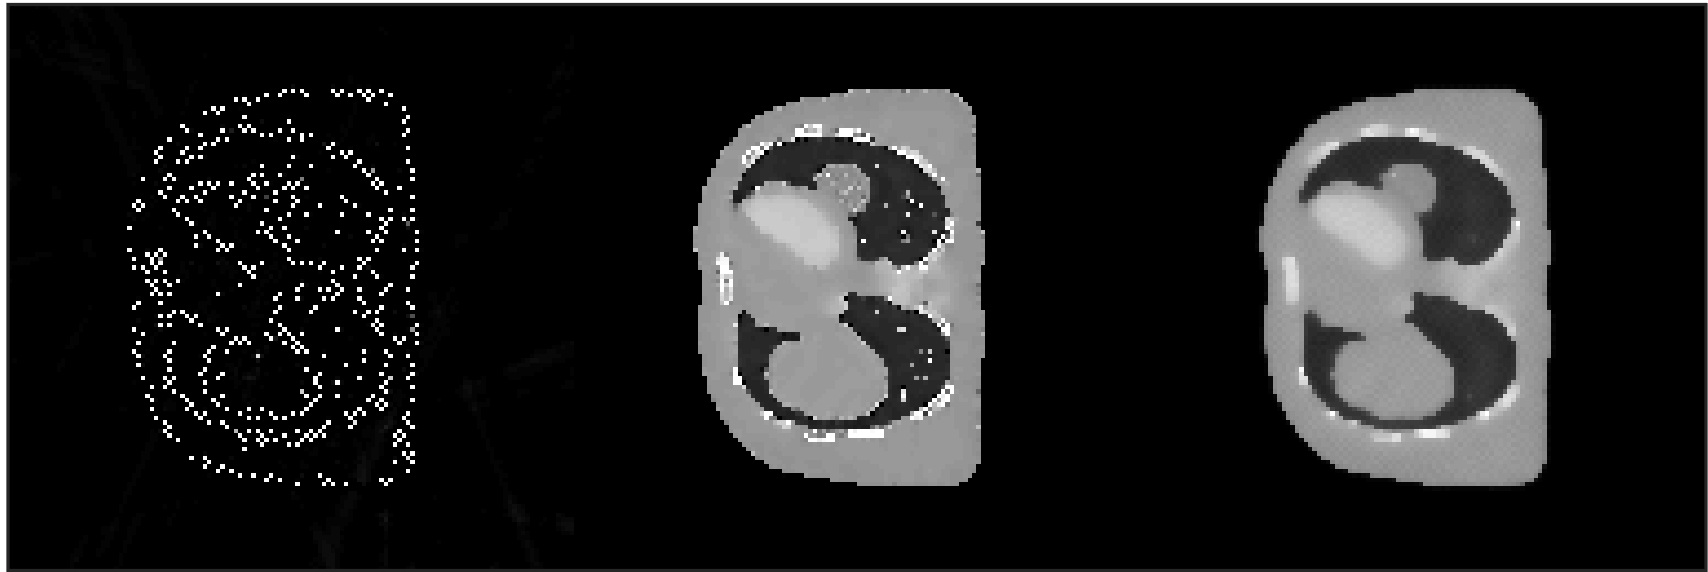
\includegraphics[width=0.7\textwidth]{Applications/TVs3.png} };
%\path (A.south west) -- (A.north west) node[pos=.18, above, rotate=90] {ASD-POCS} node[pos=.5, above, rotate=90] {b-ASD-POCS-$\beta$} node[pos=.82, above, rotate=90] {FDK};
\path (A.south west) -- (A.south east) node[pos=.18, below] {(a)} node[pos=.5, below] {(b)} node[pos=.82, below] {(c)};

\end{tikzpicture}
\caption[SART-TV algorithms with different parameters]{\label{fig:SARTTVparams}SART-TV algorithms with different amount of TV iterations per SART iteration, (a) 32 iterations, (b) 40 iterations, (c) 48 iterations.}
\end{figure}



\FloatBarrier
\section{Iterative Algorithms in Different CT Applications}
This section tries to illustrate the effect of different algorithms within the TIGRE toolbox in a series of datasets. 
\subsection{Medical Head CBCT from  The Christie Hospital}
\subsection{Cryo Soft X-Ray Tomography at Diamond Light Source}

Cryo soft X-ray tomography (Cryo-SXT) is a relatively new[CITE] technology to image micrometer size biological samples in full 3D. Generally, cell-imaging is performed with electron microscopy (EM) machines and all its variants (transmission electron microscopy, scanning electron microscopy, cryo-electron microscopy, electron tomography, etcetera), however these techniques have very limited penetration (less than 1$\mu$m) and thus often require slicing of the samples for volumetric imaging. Cryo-SXT uses the so called water window for X-ray energies around the 500eV energy range. Unlike in higher energies, where everything is invisible, water becomes transparent but carbon-based tissues are clearly visible on that range. Thus, while with lower resolution than most EM, cryooSXT allows for full volumetric visualization of the cells without damaging the samples. In order to be able to image in the extremely accurate setup in both sample handling and X-ray parameters, these cryoSXT images are captured in synchrotron facilities. The data used in this work is from the B24 beam-line at the Diamond Light Source.

However, cryoSXT data has several sources of errors that make its reconstructed images significantly noisy. The typical penetration depth of soft X-rays is around 10$\mu$m, while the samples are generally an order of magnitude bigger than that in height and width. Thus cryoSXT is a limited angle problem, where most of the datasets are sampled over a 120 degrees arc. In the extrema of this range, the images in the detector tend to have little or none information in some parts of the image due to photons not reaching the detector. Additionally, the low intensity and small sample size do mean that there the detector data is very noisy, as photons spread out more (in pixel dimension) and less photons reach the detector. The size of the sample also comes with errors in the mechanical systems of the imaging set up. When working in a scale of microns, any small vibration is visible and considerably offsets/perturbs the measured data. Generally this type of errors are removed by pre-processing using alignment techniques, but the algorithms involved are often not fault proof, and the data used in reconstruction ends up having some misalignment errors. Few of these errors can be seen in the sinogram of the dataset labelled as ``2017\_0207\_Trypanosoma\_33'', on where misalignment and missing data problems are visually perceptible.


